\chapter{Entwicklung}
\label{chap:entwicklung}
In diesem Kapitel wird die Vorgehensweise und die Realisierung der Entwicklung dokumentiert.
\section{Sprint Planung}
\label{sec:sprintplanung}
Wir haben uns entschieden das Projekt in Sprints zu unterteilen. Diese Art der Planung erschien uns am praktischsten, da wir so einen guten Überblick hatten wann was fällig ist. Die Sprintplanung wurde im Gitlab integrierten Board gemacht. Zu jeder Userstory wurde ein Issue erstellt und auf die jeweiligen Sprints verteilt.
\begin{figure}[H]
	\centering
		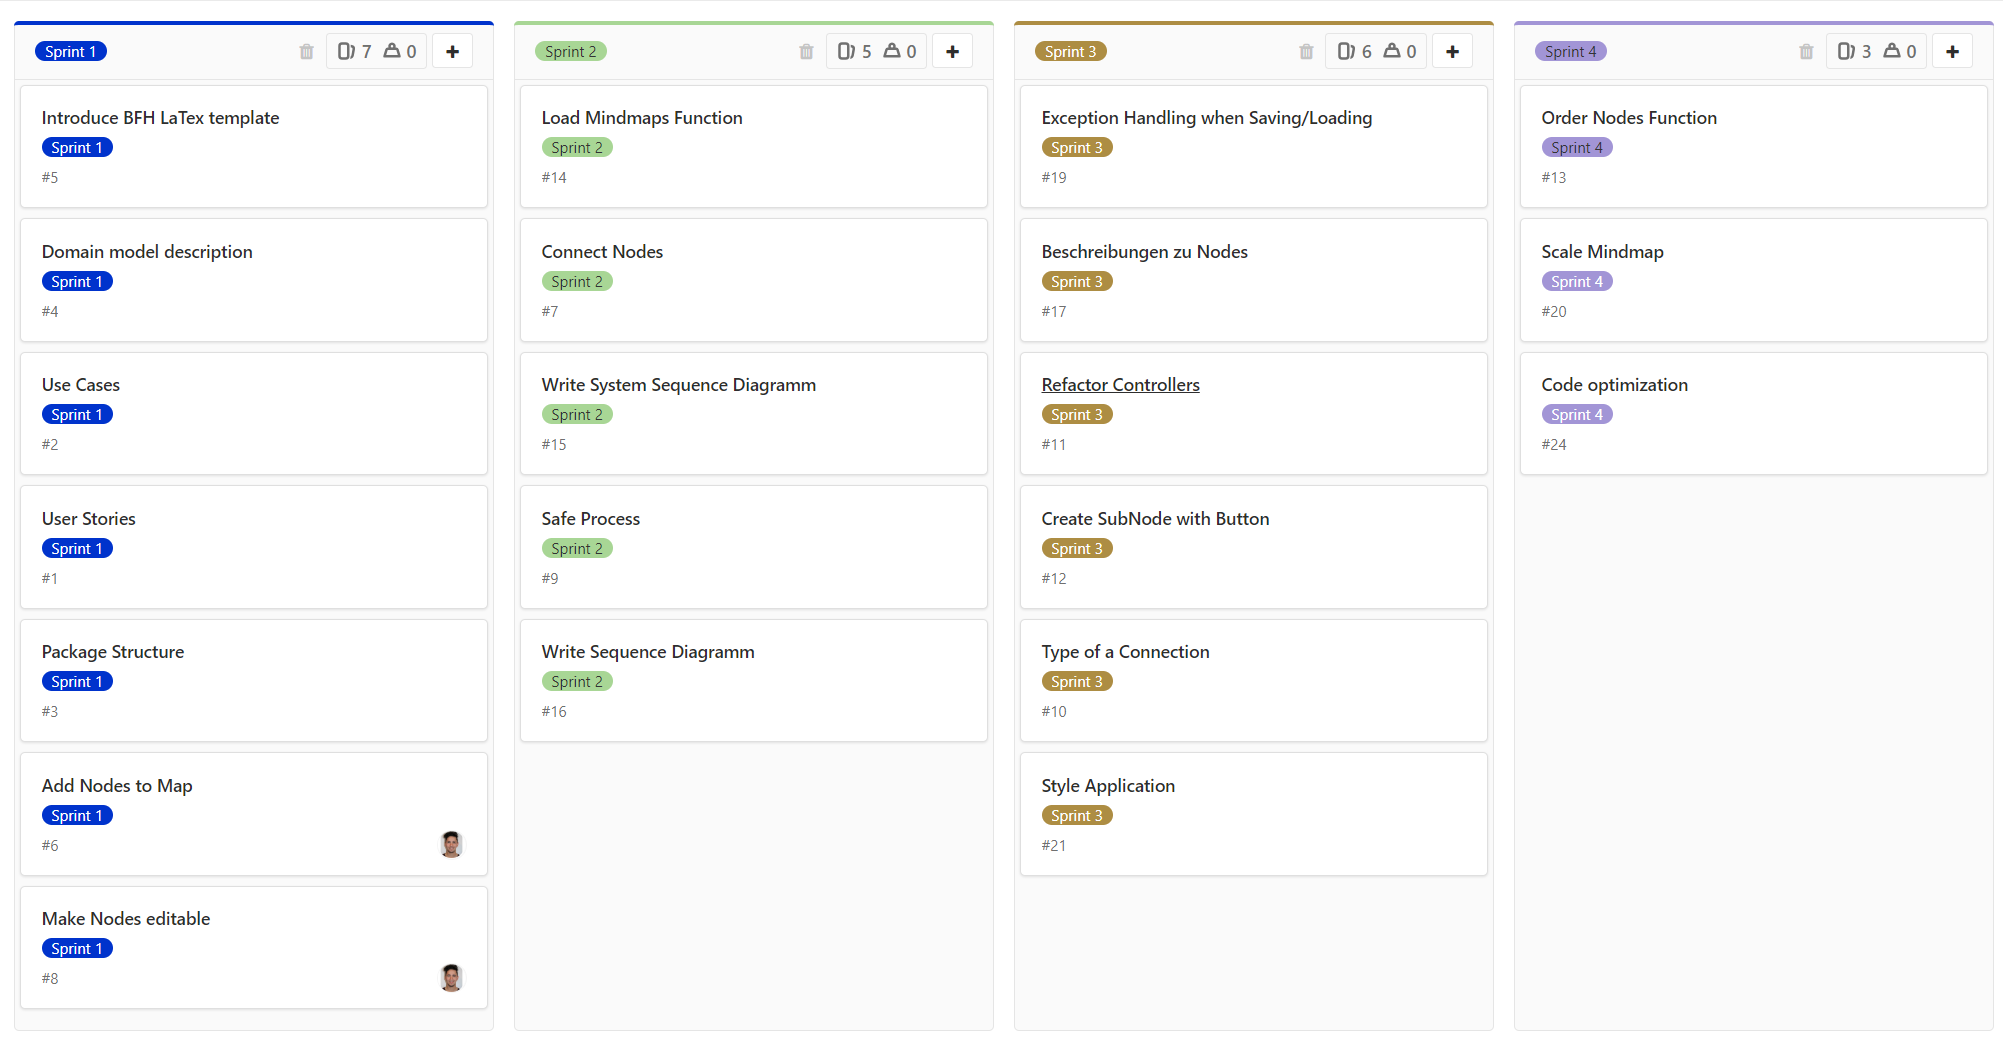
\includegraphics[width=\textwidth]{images/Board.PNG}
	\caption{Sprint Plannung}
	\label{fig:sprint_plannung}
\end{figure}

\section{Sprint 1}
\label{sec:sprint_1}
Der Sprint 1 dauerte vom 13.03 - 03.04. In diesem Sprint haben wir primär den Fokus auf die Dokumentation und die Planung gelegt. Ebenfalls haben wir uns entschieden eine Desktop Applikation zu schreiben mit JavaFX. Zusätzlich wurde ein kleiner Prototyp des Programmes erstellt. Erste Funktionen wie das Erstellen von Knoten und deren Verschiebung wurde ebenfalls realisiert.
\section{Sprint 2}
\label{sec:sprint_2}
Der Sprint 2 dauerte vom 03.04 - 24.04. In diesem Sprint wurde dann richtig begonnen mit dem Programmieren der Funktionalitäten. Es wurden ebenfalls die SD/SSD Diagramme erstellt. Realisiert wurden die Funktionen zum Verbinden von Knoten und das Laden und Speichern der Knoten. Zum Laden und Speichern der Knoten haben wir uns für JAXB for Java entschieden. Dieses Framework erlaubt es aus Objekten XML Dateien zu erstellen.
In diesem Sprint haben wir bemerkt, dass unser Programm zu unübersichtlich wird, wir haben unsere Kontrollerstruktur daraufhin angepasst.
\section{Sprint 3}
\label{sec:sprint_3}
Der Sprint 3 dauert vom 24.04 - 15.05. In diesem Sprint wurde vor allem zuerst ein grosses Refactoring des Codes gemacht. Der Hauptkontroller wurde in 3 Unterkontroller geteilt. Dies gab dem Programm mehr Lesbarkeit und war infolgedessen auch einfacher zu erweitern. Ebenfalls wurde das Feature zur Zusatzinformation für Knoten, der Unterknoten Button und der Typ einer Verbindung hinzugefügt. Am Schluss des Sprints wurde dann noch die Applikation optisch verschönert.
\section{Sprint 4}
\label{sec:sprint_4}
Der Sprint 4 dauert vom 15.05 - 29.05. In diesem Sprint wurde das Programm beendet. Diverse Bugs wurden ausgebessert und einzelne neue Funktionen wie das Skalieren der Applikation und die ordnen Funktion wurde hinzugefügt. 

\section{Kontroller Management}
\label{sec:controller_mgmnt}
Das Programm besitzt 4 Kontroller, die jeweils einer FXML Datei zugeordnet sind. Der MainController ist dabei die Schnittstelle zwischen der View und den Kontrollern. Der CanvasController ist für alle Aktionen im Programmfeld zuständig, er erstellt zum Beispiel neue Knoten oder färbt diese. Der MenuBarController ist für die Aktionen in der Menubar zuständig, er speichert und lädt die Maps. Zuletzt noch der ToolbarController, dieser prüft primär welche Aktionen im CanvasController ausgeführt werden sollen, wie z.b. Knoten erstellen, Verbinden usw.

\section{Ordnungs Funktion}
\label{sec:controller_mgmnt}
Die Knoten Ordnen Funktion wurde implementiert um dem Benutzer zu helfen sein Mindmap aufzuräumen.
Die Funktion kann dabei 3 Probleme erkennen. 
\begin{figure}[H]
	\centering
		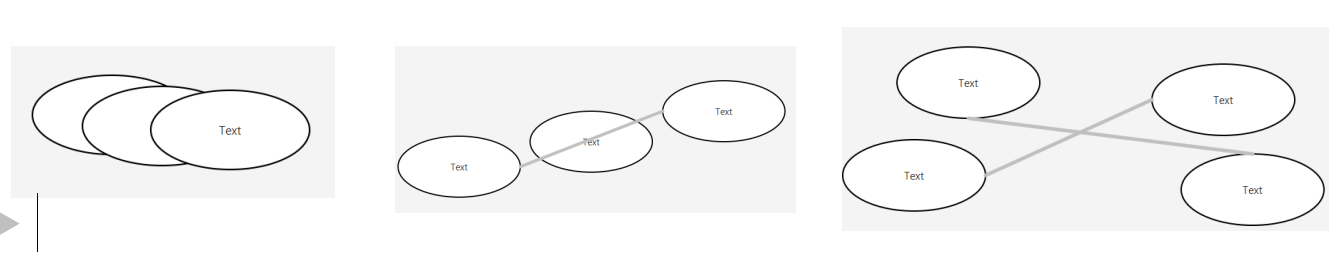
\includegraphics[width=\textwidth]{images/threeissues.PNG}
	\caption{3 erkennbare Probleme}
	\label{fig:probleme}
\end{figure}

Diese 3 Probleme versucht nun der Algorithmus zu lösen. Er geht dabei nach einem Try and Error konzept vor. Es wird versucht den Knoten in 8 Richtungen zu verschieben und geprüft ob das Problem gelöst wurde. Falls nicht, wird die Distanz bis auf 7x vergrössert. Die Distanz des Verschiebens ist jeweils der Radius der zu verschiebenden Ellipse. 

\begin{figure}[H]
	\centering
		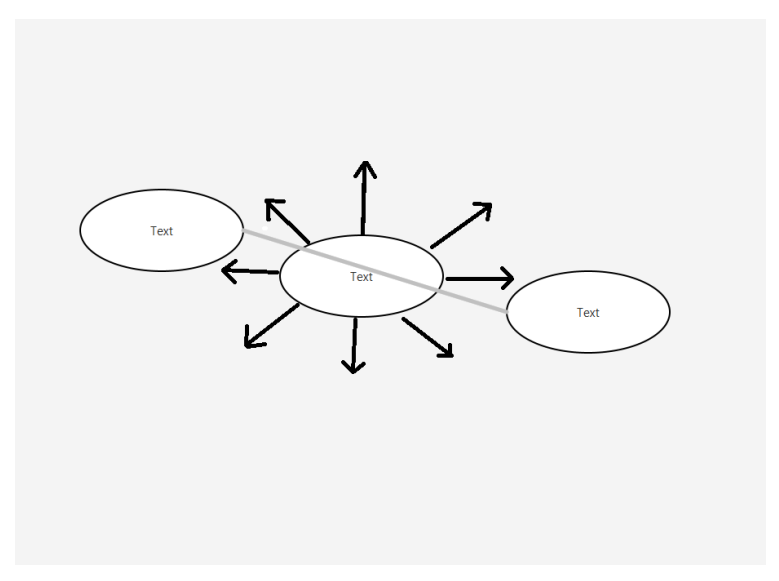
\includegraphics[scale=0.5]{images/solving.PNG}
	\caption{Problemlösung}
	\label{fig:problemloesung}
\end{figure}

Das Fazit zu dieser Lösung ist, dass der Algorithmus bei einfachen Problemen ohne Probleme eine Lösung findet. Bei schwereren Problemen jedoch findet er teils keine Lösung. Ebenfalls ist der Algorithmus sehr ineffizient und kann lange dauern wenn sehr viele Knoten geprüft werden müssen. 

\section{Programm ausführen}
\label{sec:run_program}

\subsection{Tools and Software}
\label{subsec:tools}
Unsere Mindmap Applikation benutzt folgende Software und Frameworks.
\begin{itemize}
\item Java jdk1.8.0\_{}191
\item JavaFX http://javafx.com/javafx/8.0.191
\item JavaFX Scene Builder 10.0.0
\end{itemize}

\subsection{Installation}
Um das Programm auszuführen muss zu erst das Repository per Git geklont werden.
\begin{verbatim}
git clone https://gitlab.ti.bfh.ch/rascl1/mindmap.git
\end{verbatim}
Wenn das Projekt in ein IDE importiert wird, muss der Ordner "{}MindMap"{} als Grundlage gewählt werden.\\
Oder das Programm kann mit der \texttt{MindMap.jar} ausgeführt werden.